\chapter{Основное содержание работы}
\textbf{Введение} содержит обоснование актуальности научных исследований, изложенных в диссертации,
а также сформулированные цели, научную новизну, практическую и теоретическую ценность диссертационной работы.

\textbf{В первой главе} описываются конструкция и принципы движения квадрокоптера,
рассмотрены подходы к построению модели динамики квадрокоптера и возможные постановки задачи управления,
дан аналитический обзор основных методов, используемых для синтеза контура управления квадрокоптером;
также приведены примеры усовершенствования конструкции стандартного квадрокоптера,
для некоторых из них подробно рассмотрено влияние модификаций на динамику системы.

Основными элементами конструкции стандартного квадрокоптера являются корпус и четыре двигателя с прикрепленными к ним пропеллерами. Вертикальное движение аппарата обусловлено изменением общей тяги всех двигателей. Горизонтальное движение совершается за счет изменения направления вектора тяги вследствие наклона корпуса БЛА. Таким образом, независимыми параметрами движения являются положение и угол рысканья квадрокоптера.

Движение центра масс БЛА определяется силами гравитации, аэродинамического сопротивления и тягой пропеллеров
\begin{equation} \label{eq:common_traslational_motion}
M \ddot{\bm{r}} = \bm{F}_g + \bm{F}_{aero} + \bm{F}_{thr}.
\end{equation}
Здесь, 
\begin{equation} \label{eq:gravity_force}
\bm{F}_g = M\bm{g},
\end{equation}
\begin{equation} \label{eq:aerodynamic_force}
\bm{F}_{aero} = - \frac{1}{2} \rho_{air} C S_{\perp} |\dot{\bm{r}}| \dot{\bm{r}},
\end{equation}
\begin{equation} \label{eq:thrust_force}
\bm{F}_{thr} = \sum_{i=1}^{4}{ { k \tilde\omega^2_i \bm{z}_i}.}
\end{equation}
Основными параметрами, определяющими движение центра масс БЛА являются общая масса {$M$} конструкции, ускорение свободного падения \bm{$g$}, плотность среды {$\rho_{air}$}, аэродинамические свойства корпуса аппарата и пропеллеров; $\tilde\omega_i$ -- обороты $i$-го пропеллера, $\bm{z_i}$ -- ось его вращения.

Вращательное движение корпуса БЛА определяется моментами сил, которые создают двигатели с пропеллерами и гироскопическим моментом самого корпуса
\begin{equation} \label{eq:common_rotational_motion}
\bm{J}_B\dot{\bm{\Omega}}_B + \bm{\Omega}_B \times  \bm{J}_B{\bm{\Omega}_B} = \sum_{i=1}^{4}{\bm{\tau}_{Bi}}.
\end{equation}

Использование поворотных роторов позволяет расширить вектор управляющих воздействий, благодаря чему для движения квадрокоптера в каком-либо направлении нет необходимости наклонять корпус, таким образом можно достичь независимого управления по положению и ориентации.

\begin{figure}[H]
	\centering
	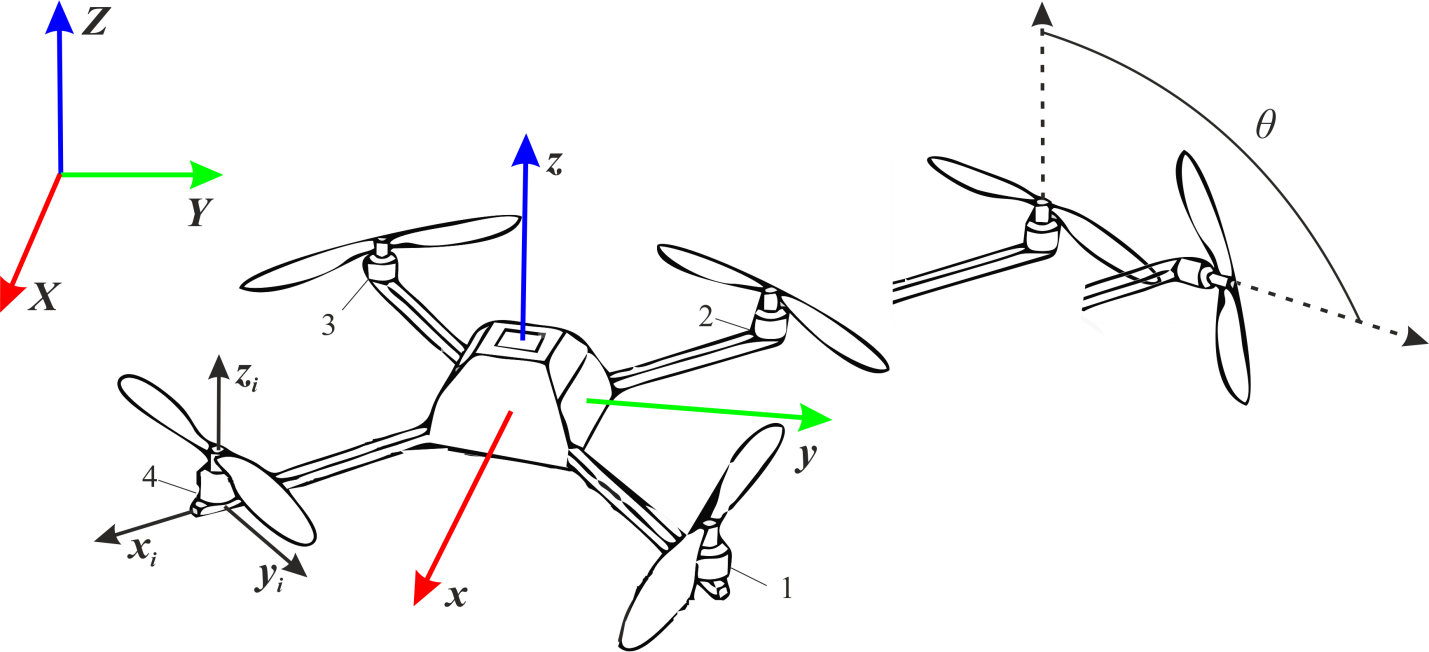
\includegraphics[scale=0.9]{tiltrotor_scheme}
	\caption{ -- Общая схема квадрокоптера с поворотными роторами}
	\label{fig:tiltrotor_scheme}
\end{figure}

\textbf{Во второй главе} рассматривается управляемая динамика квадрокоптера с поворотными роторами. Наличие дополнительных сервоприводов усложняет модель движения БЛА \eqref{eq:common_traslational_motion} - \eqref{eq:common_rotational_motion}, делая его зависящим от текущей геометрии аппарата и скорости ее изменения

\begin{equation} \label{eq:m_traslational_motion}
M \ddot{\bm{r}} = M \bm{g}^I - \frac{1}{2} \rho C S_{\perp} |\bm{v}^I| \bm{v}^I + \sum_{i=1}^{4}{ { (-1)^{i+1} k \tilde \omega_i |\tilde \omega_i| \bm{e}^I_{z_i}}(\theta_i)},
\end{equation}

\begin{equation} \label{eq:m_final_rotational_motion}
\begin{aligned}
\bm{J}_B\dot{\bm{\Omega}}^B + \bm{\Omega}^B \times \bm{J}_B{\bm{\Omega}^B} =
&\sum_{i=1}^{4} {\bm{r}^B_i \times
	(-1)^{i+1} k \tilde \omega_i |\tilde \omega_i| \bm{e}^I_{z_i}} - \\
-\sum_{i=1}^{4} {b \tilde \omega_i |\tilde \omega_i| \bm e^{R_i}_{r_i}} +
&\sum_{i=1}^{4} q_{ B {R_i}} \circ (\bm{J}_{R_i}\dot{\bm{\omega}}^{R_i}_i + \bm{\omega}^{R_i}_i \times \bm{J}_{R_i}{\bm{\omega}^{R_i}_i}) \circ \tilde q_{ B {R_i}}
,
\end{aligned}
\end{equation}
где полная угловая скорость $\bm{\omega}^{R_i}_i$ $i$-того ротора с пропеллером
\begin{equation} \label{eq:m_prop_ang_vel}
\bm{\omega}^{R_i}_i =
q_{{R_i} B} \circ (\bm{\Omega}^B + \dot {\theta}_i \bm e^B_{r_i}) \circ \tilde {q}_{{R_i}B} +
\tilde \omega_i \bm{e}^{R_i}_{z_i}
.
\end{equation}

Считая заданной требуемую траекторию БЛА в координатном пространстве, положим целью управления обеспечение наперёд заданной траектории центра масс аппарата, а также требуемой ориентации. В качестве переменных управления выберем скорости вращения пропеллеров ${\tilde \omega}_i$ и углы поворота роторов ${\theta}_i$:
\begin{equation} \label{eq:m_ctrl_out}
\begin{aligned}
&\bm{u} = (\bm \omega_u, \bm \theta_u)^T,
\\
\bm \omega_u =
(\tilde\omega_1 |\tilde\omega_1|,
\tilde\omega_2 |\tilde\omega_2|&,
\tilde\omega_3 |\tilde\omega_3|,
\tilde\omega_4 |\tilde\omega_4|)^T,
\quad
\bm \theta_u = (\theta_1, \theta_2 , \theta_3 , \theta_4 )^T.
\end{aligned}
\end{equation}
Регуляторы, обеспечивающие необходимое управление по положению и ориентации могут быть построены, как
\begin{equation} \label{eq:m_reg}
\begin{aligned}
\ddot{\bm{r}_d}(t)&=
\ddot{\bm{r}}^0(t)+\bm{K}_{r1}(\dot{\bm{r}}^0(t) - \dot{\bm{r}}(t))+\bm{K}_{r2}\delta \bm r,\\
\dot{\bm{\Omega}}_d(t)&=
\dot{\bm{\Omega}}^0(t)+\bm{K}_{\Omega1}(\bm{\Omega}^0(t)-\bm{\Omega}(t))+\bm{K}_{\Omega2}\delta\bm{q},
\end{aligned}
\end{equation}

Реализация контура управления с регуляторами (\ref{eq:m_reg}) требует обращения динамики системы, то есть определения значений всех управляющих параметров (\ref{eq:m_ctrl_out}) по выходу из регулятора (\ref{eq:m_reg}).
Для достижения этой цели преобразуем уравнения модели (\ref{eq:m_traslational_motion}), (\ref{eq:m_final_rotational_motion}).
\begin{equation} \label{eq:m_dyn}
\begin{aligned}
&\bm F(\ddot{\bm r}_d, \dot{\bm r}, q) = k F_{thr} (\bm \theta_u) \bm \omega_u,\\
&\bm T(\dot{\bm \Omega}_d, \bm\Omega) = \Big(
kLT_{thr}(\bm\theta_u) - bT_{aero}(\bm\theta_u)
\Big)
\bm \omega_u.
\end{aligned}
\end{equation}

Система (\ref{eq:m_dyn}) недоопределена и нелинейна относительно компонент $\bm \theta_u$, что значительно затрудняет ее аналитическое решение. Доопределим систему, используя выражения для распределения вертикальных составляющих сил и моментов между парами двигателей, расположенных на параллельных лучах
\begin{equation} \label{eq:m_dyn_balance_1}
\begin{aligned}
&k \tilde\omega_1 |\tilde\omega_1| c_1 + k \tilde\omega_3 |\tilde\omega_3| c_3 =
\frac{1}{2} \bm F_z + \varepsilon_F,
\\
&\tilde\omega_1 |\tilde\omega_1| (bc_1 - kLs_1)
+ \tilde\omega_3 |\tilde\omega_3| (bc_3 - kLs_3) =
\frac{1}{2} \bm T_z + \varepsilon_T,
\end{aligned}
\end{equation}

\begin{equation} \label{eq:m_dyn_balance_2}
\begin{aligned}
&k \tilde\omega_2 |\tilde\omega_2| c_2 + k \tilde\omega_4 |\tilde\omega_4| c_4 =
-\frac{1}{2} \bm F_z + \varepsilon_F,
\\
&\tilde\omega_2 |\tilde\omega_2| (bc_2 + kLs_2)
+ \tilde\omega_4 |\tilde\omega_4| (bc_4 + kLs_4) =
\frac{1}{2} \bm T_z - \varepsilon_T,
\end{aligned}
\end{equation}
где $\varepsilon_F$ и $\varepsilon_F$ -- балансировочные параметры.
Полученная система уравнений (\ref{eq:m_dyn}), (\ref{eq:m_dyn_balance_1}) имеет аналитическое решение:
\begin{equation} \label{eq:m_dyn_resolve}
\begin{aligned}
&\tilde\omega_i |\tilde\omega_i| =
\frac{(-1)^{i+1}}{2kL}\sqrt{
	A^2_i + 
	B^2_i
},
\\
\phantom{}
\\
&\theta_i = 
2 \text{arctg} \Bigg[(-1)^{i+1}	
\frac{A_i -
	\sqrt{
		A^2_i + 
		B^2_i
}}
{B_i}
\Bigg],
\end{aligned}
\end{equation}
где $A_i = A_i(\bm F, \bm T, \varepsilon_F, \varepsilon_T)$
и
$B_i = B_i(\bm F, \bm T, \varepsilon_F, \varepsilon_T)$
-- скалярные функции, куда линейно входят компоненты левой части уравнений динамики \eqref{eq:m_dyn}
$\bm F(\ddot{\bm r}_d, \dot{\bm r}, q)$
и
$\bm T(\dot{\bm \Omega}_d, \bm\Omega)$.
Таким образом, полученное решение связывает выход регулятора с управляющими параметрами при наличии обратной связи, а именно известных текущих координате $\bm r^I$, скорости $\bm v^I$, ориентации $q_{IB}$ и угловой скорости $\bm \Omega^B$.

Анализ решения \eqref{eq:m_dyn_resolve} позволяет ограничить выход регулятора \eqref{eq:m_reg} таким образом, чтобы компоненты вектора управляющих воздействий не выходили за пределы заданных значений 
\begin{equation} \label{eq:m_limits_init}
\begin{aligned}
&0< (-1)^{i+1} \tilde \omega_i |\tilde\omega_i| < \tilde \omega_{max}^2,
\\
&|\theta_i| < \theta_{max} < \pi,
\end{aligned}
\end{equation}
что позволяет учесть ограничения на физические параметры исполнительных органов системы управления.

Затем рассматривается сценарий потери аппаратом двух смежных двигателей; показано, что наличие поворотных роторов может спасти аппарат от неконтролируемого падения и обеспечить мягкую посадку.



\textbf{Третья глава} посвящена реализации обратных связей в контуре управления. Для реализации обратных связей в контуре управления необходимо обеспечить оценку текущего положения, скорости, кватерниона ориентации и угловой скорости БЛА. Получить данные оценки можно с помощью стандартного набора бортовых датчиков, обычно включающего в себя спутниковую систему глобального позиционирования, цифровой барометрический датчик давления, трехосевые электромеханические акселерометр и гироскоп, а также магнитный компас. Однако в связи с высокими требованиями к массово-габаритным параметрам бортовой системы навигации для небольших летательных аппаратов бортовые измерения имеют ограничения по качеству. Высокий уровень шума побуждает использовать алгоритмы оценки состояния, способные значительно понизить его уровень.

Для выбора подходящего алгоритма фильтрации было проведено исследование, где были рассмотрены  алгоритмы расширенного фильтра Калмана (extended Kalman filter, EKF) и несколько вариантов реализации сигма-точечного фильтра Калмана (unscented Kalman filter, UKF). Приводится описание принципов работы EKF, UKF, а также одной из частных реализаций сигма-точечного фильтра -- кубатурного фильтра Калмана (cubature Kalman filter, CKF) и описаны особенности применения этих алгоритмов для оценки состояния квадрокоптера с поворотными роторами.

Для сравнения производительности методов проведены вычислительные эксперименты.
Предложенные во второй главе алгоритмы использовались для управления БЛА, в качестве целевых траекторий выбраны трехмерные кривые в пространстве, параметры которых генерировались случайным образом в известных пределах. В качестве параметра, определяющего производительность фильтров,
выбрано среднеквадратичное отклонение компонент вектора оценки состояния от результатов интегрирования уравнений движения.
Для исключения влияния параметров конкретной целевой траектории на результаты эксперимента среднеквадратичное отклонение усредняется по 100 пролетам.
На графике ниже (рис. \ref{fig:est_cmpr}) представлена зависимость усредненного среднеквадратичного отклонения от интервала проводимых измерений $T_N = N\delta$ для высоты, вертикальной скорости, угла рысканья и скорости его изменения.

\begin{figure}[H]
	\begin{minipage}[h]{0.49\linewidth}
		\center{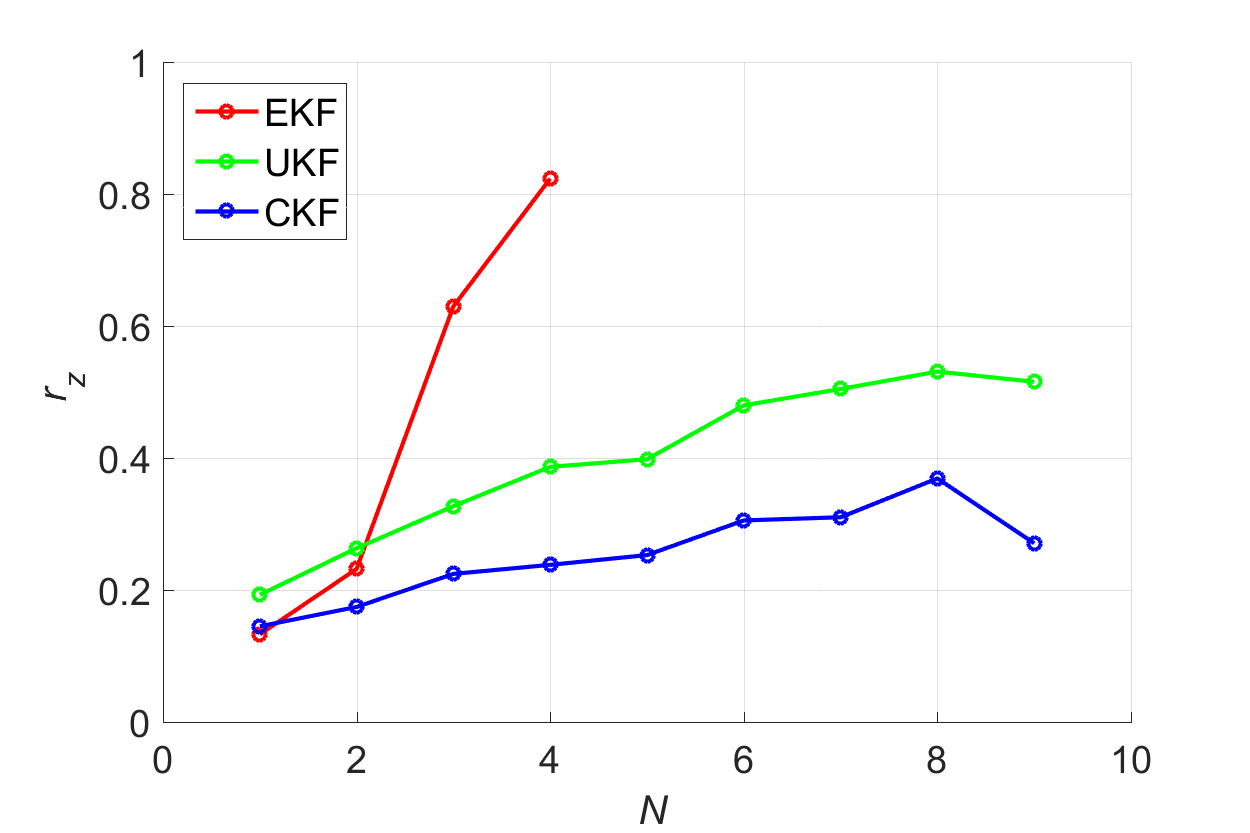
\includegraphics[height=0.2\textheight]{estcmpr_1} \\ а)}
	\end{minipage}
	\hfill
	\begin{minipage}[h]{0.49\linewidth}
		\center{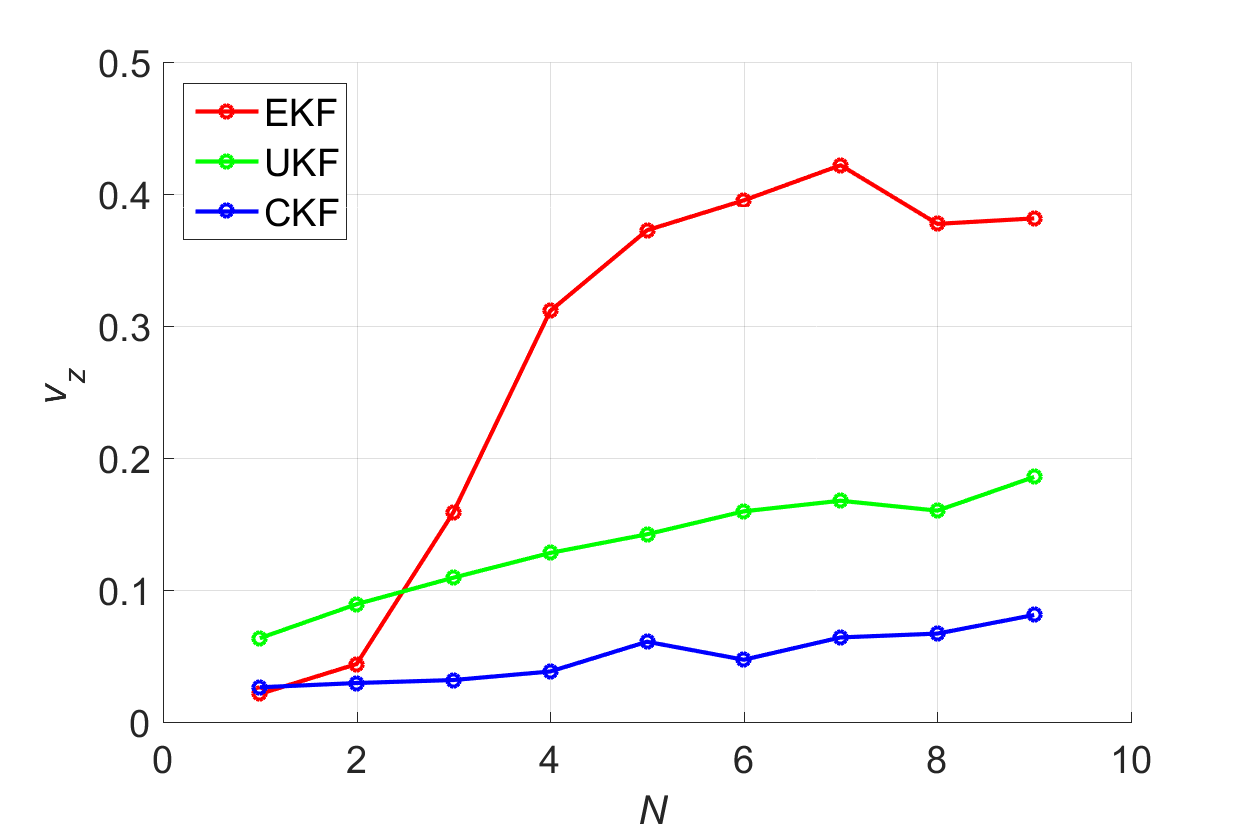
\includegraphics[height=0.2\textheight]{estcmpr_2} \\ б)}
	\end{minipage}
	\\
	\begin{minipage}[h]{0.49\linewidth}
		\center{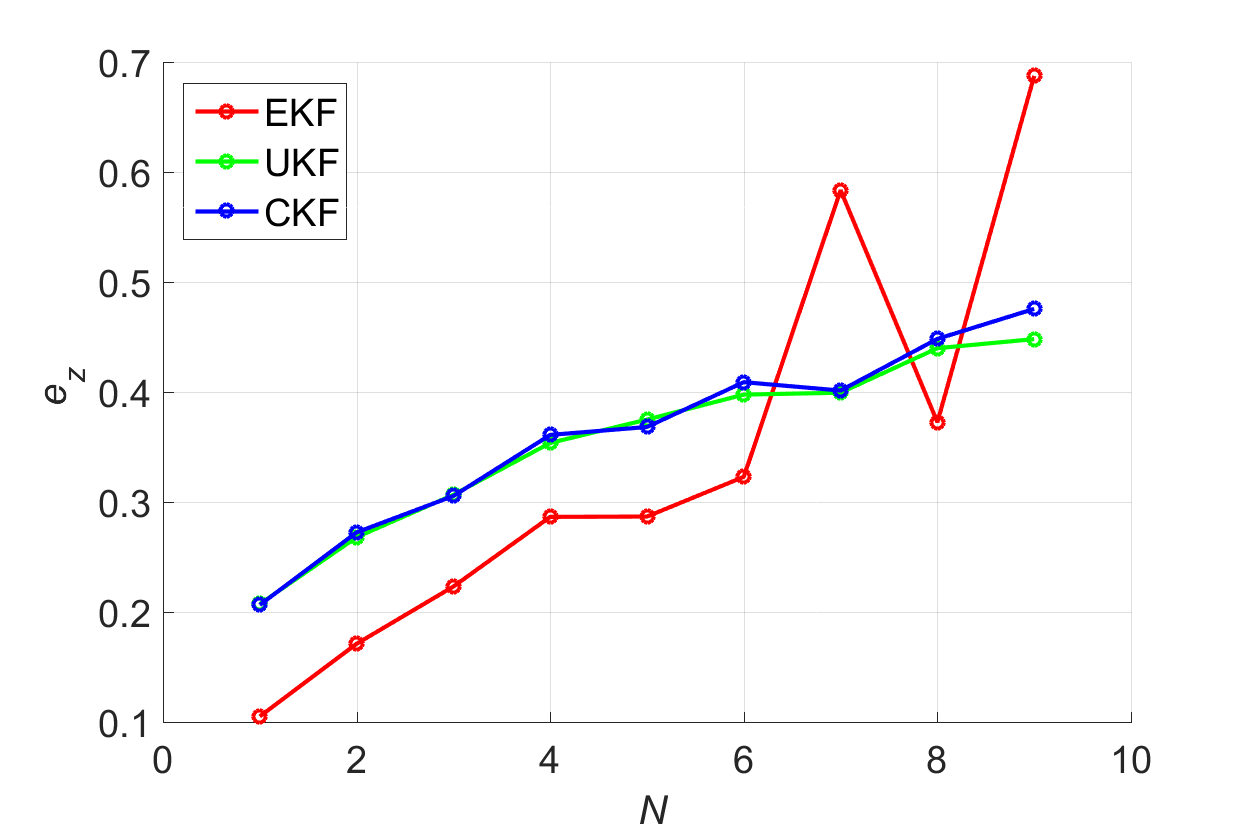
\includegraphics[height=0.2\textheight]{estcmpr_3} \\ а)}
	\end{minipage}
	\hfill
	\begin{minipage}[h]{0.49\linewidth}
		\center{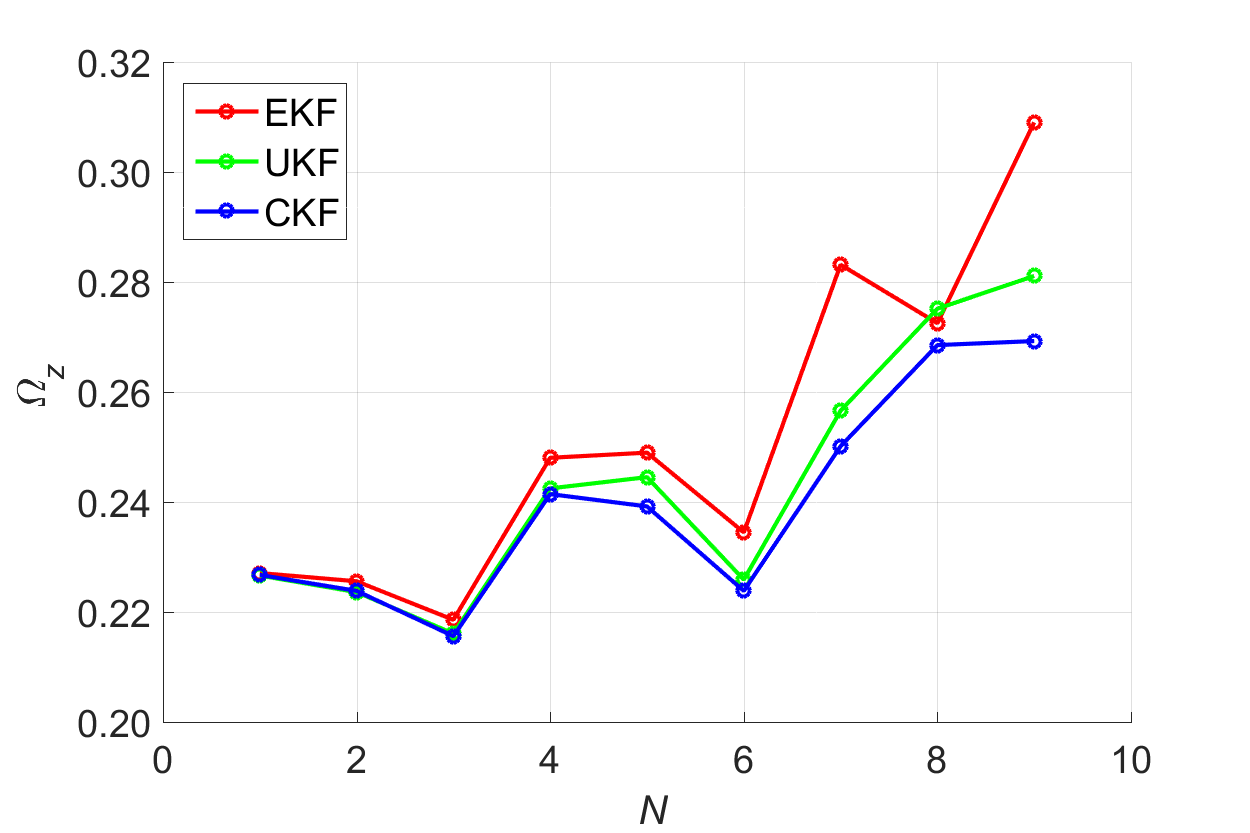
\includegraphics[height=0.2\textheight]{estcmpr_4} \\ б)}
	\end{minipage}
	\caption{Сравнение производительности алгоритмов фильтрации}
	\label{fig:est_cmpr}
\end{figure}

Качество оценки вектора состояния коррелирует с интервалом работы фильтров --
снижение частоты измерений  ведет к ухудшению параметров оценки.
Наиболее низкую производительность на больших интервалах измерений показывает расширенный фильтр Калмана:
уже для $N>2$ ошибки оценки состояния в нескольких случаях выходят за рамки допустимых,
а при $N \geq 5$ оценка положения становится некорректной.
Производительность сигма-точечного и кубатурного фильтров Калмана с ростом $N$ также падает,
но не настолько заметно.
Сравнительный анализ результатов UKF и CKF показал, что CKF-алгоритм производит более точную оценку состояния
в большинстве рассматриваемых случаев и является более устойчивым к повышению интервала измерений.
Таким образом для системы управления квадрокоптером с поворотными роторами был выбран кубатурный фильтр Калмана.

\textbf{В четвертой главе} представлены результаты вычислительных экспериментов. 

В первом эксперименте аппарат должен выполнить наблюдение за подвижным объектом, летя неподалеку от него и ориентируя камеру, установленную спереди, так, чтобы объект находился в центре полученного изображения. Выбраны параметры, соответствующие небольшому квадрокоптеру, способному нести на борту дополнительную нагрузку в виде камеры высокого разрешения (Таблица \ref{tb:params_table}).
Рассчитаны ограничения на выходы регулятора
для 
$\tilde \omega_{max}$ = 1140 рад/с,
$\theta_{max}$ = ${\pi}/{3}$ рад.
\begin{table}[h!]
	\centering
	\caption{ -- Параметры модели}\label{tb:params_table} 
	\begin{tabular}{lcl}
		\hline
		Параметр & Обозначение & Значение  \\\hline
		Общая масса & $M$ & 2 кг  \\
		Тензор инерции корпуса & $\bm J_B$ & $diag(2,\ 2,\ 4)\cdot{10^{-2}}$ кг$\cdot$м$^2$  \\
		Тензор инерции ротора & $\bm J_R$ & $diag(2,\ 2,\ 1)\cdot{10^{-5}}$ кг$\cdot$м$^2$  \\
		Миделево сечение корпуса & $S_{\perp}$ & 0,12 м$^2$ \\
		Луч & $L$ & 0,25 м \\
		Аэродинамический коэффициент & $C$ & 1,05\\
		Аэродинамический коэффициент & $k$ & 1,13$\cdot 10^{-5}$ Н$\cdot$с$^2\cdot$рад$^{-2}$ \\		
		Аэродинамический коэффициент & $b$ & 1,5$\cdot 10^{-6}$ Н$\cdot$м$\cdot$с$^2\cdot$рад$^{-2}$ \\		
		Максимальные обороты & $\tilde \omega_{max}$ & 1140 рад/с \\		
		Максимальный угол & $\theta_{max}$ & ${\pi}/{3}$ рад \\
		Константа балансировки & $\varepsilon_\tau$ &6 Н$\cdot$м \\
		\hline
	\end{tabular}
\end{table}
Траектория БЛА и наблюдаемого объекта изображены на рисунке \ref{fig:mau_traj}.
\begin{figure}[H]
	\centering
	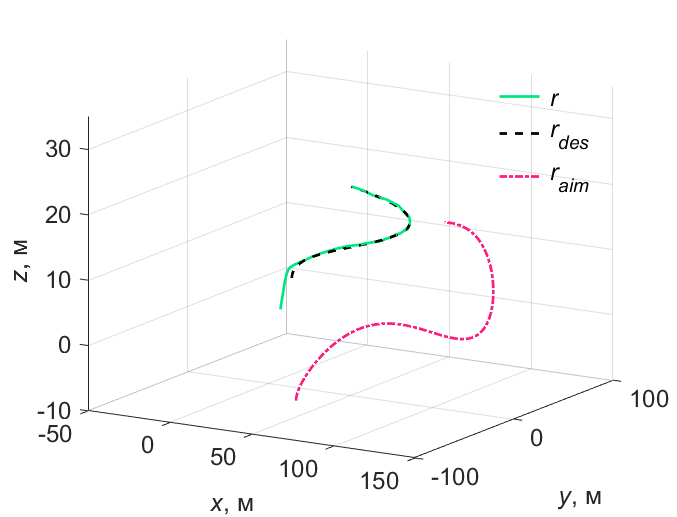
\includegraphics[width=14cm]{traj.png}
	\caption{ -- Траектория БЛА и объекта наблюдения}
	\label{fig:mau_traj}
\end{figure}

На рисунке \ref{fig:mau_errors}, на графиках слева, изображены ошибки ориентации по углам крена, тангажа и рысканья,
а справа -- ошибки положения  квадрокоптера по осям $X$, $Y$ и $Z$.
Ошибки по каждому из углов ориентации после стабилизации не превышают одного градуса.
После выхода аппарата на целевую траекторию максимальное абсолютное отклонение от траектории составило 30 см.
\begin{figure}[H]
	\centering
	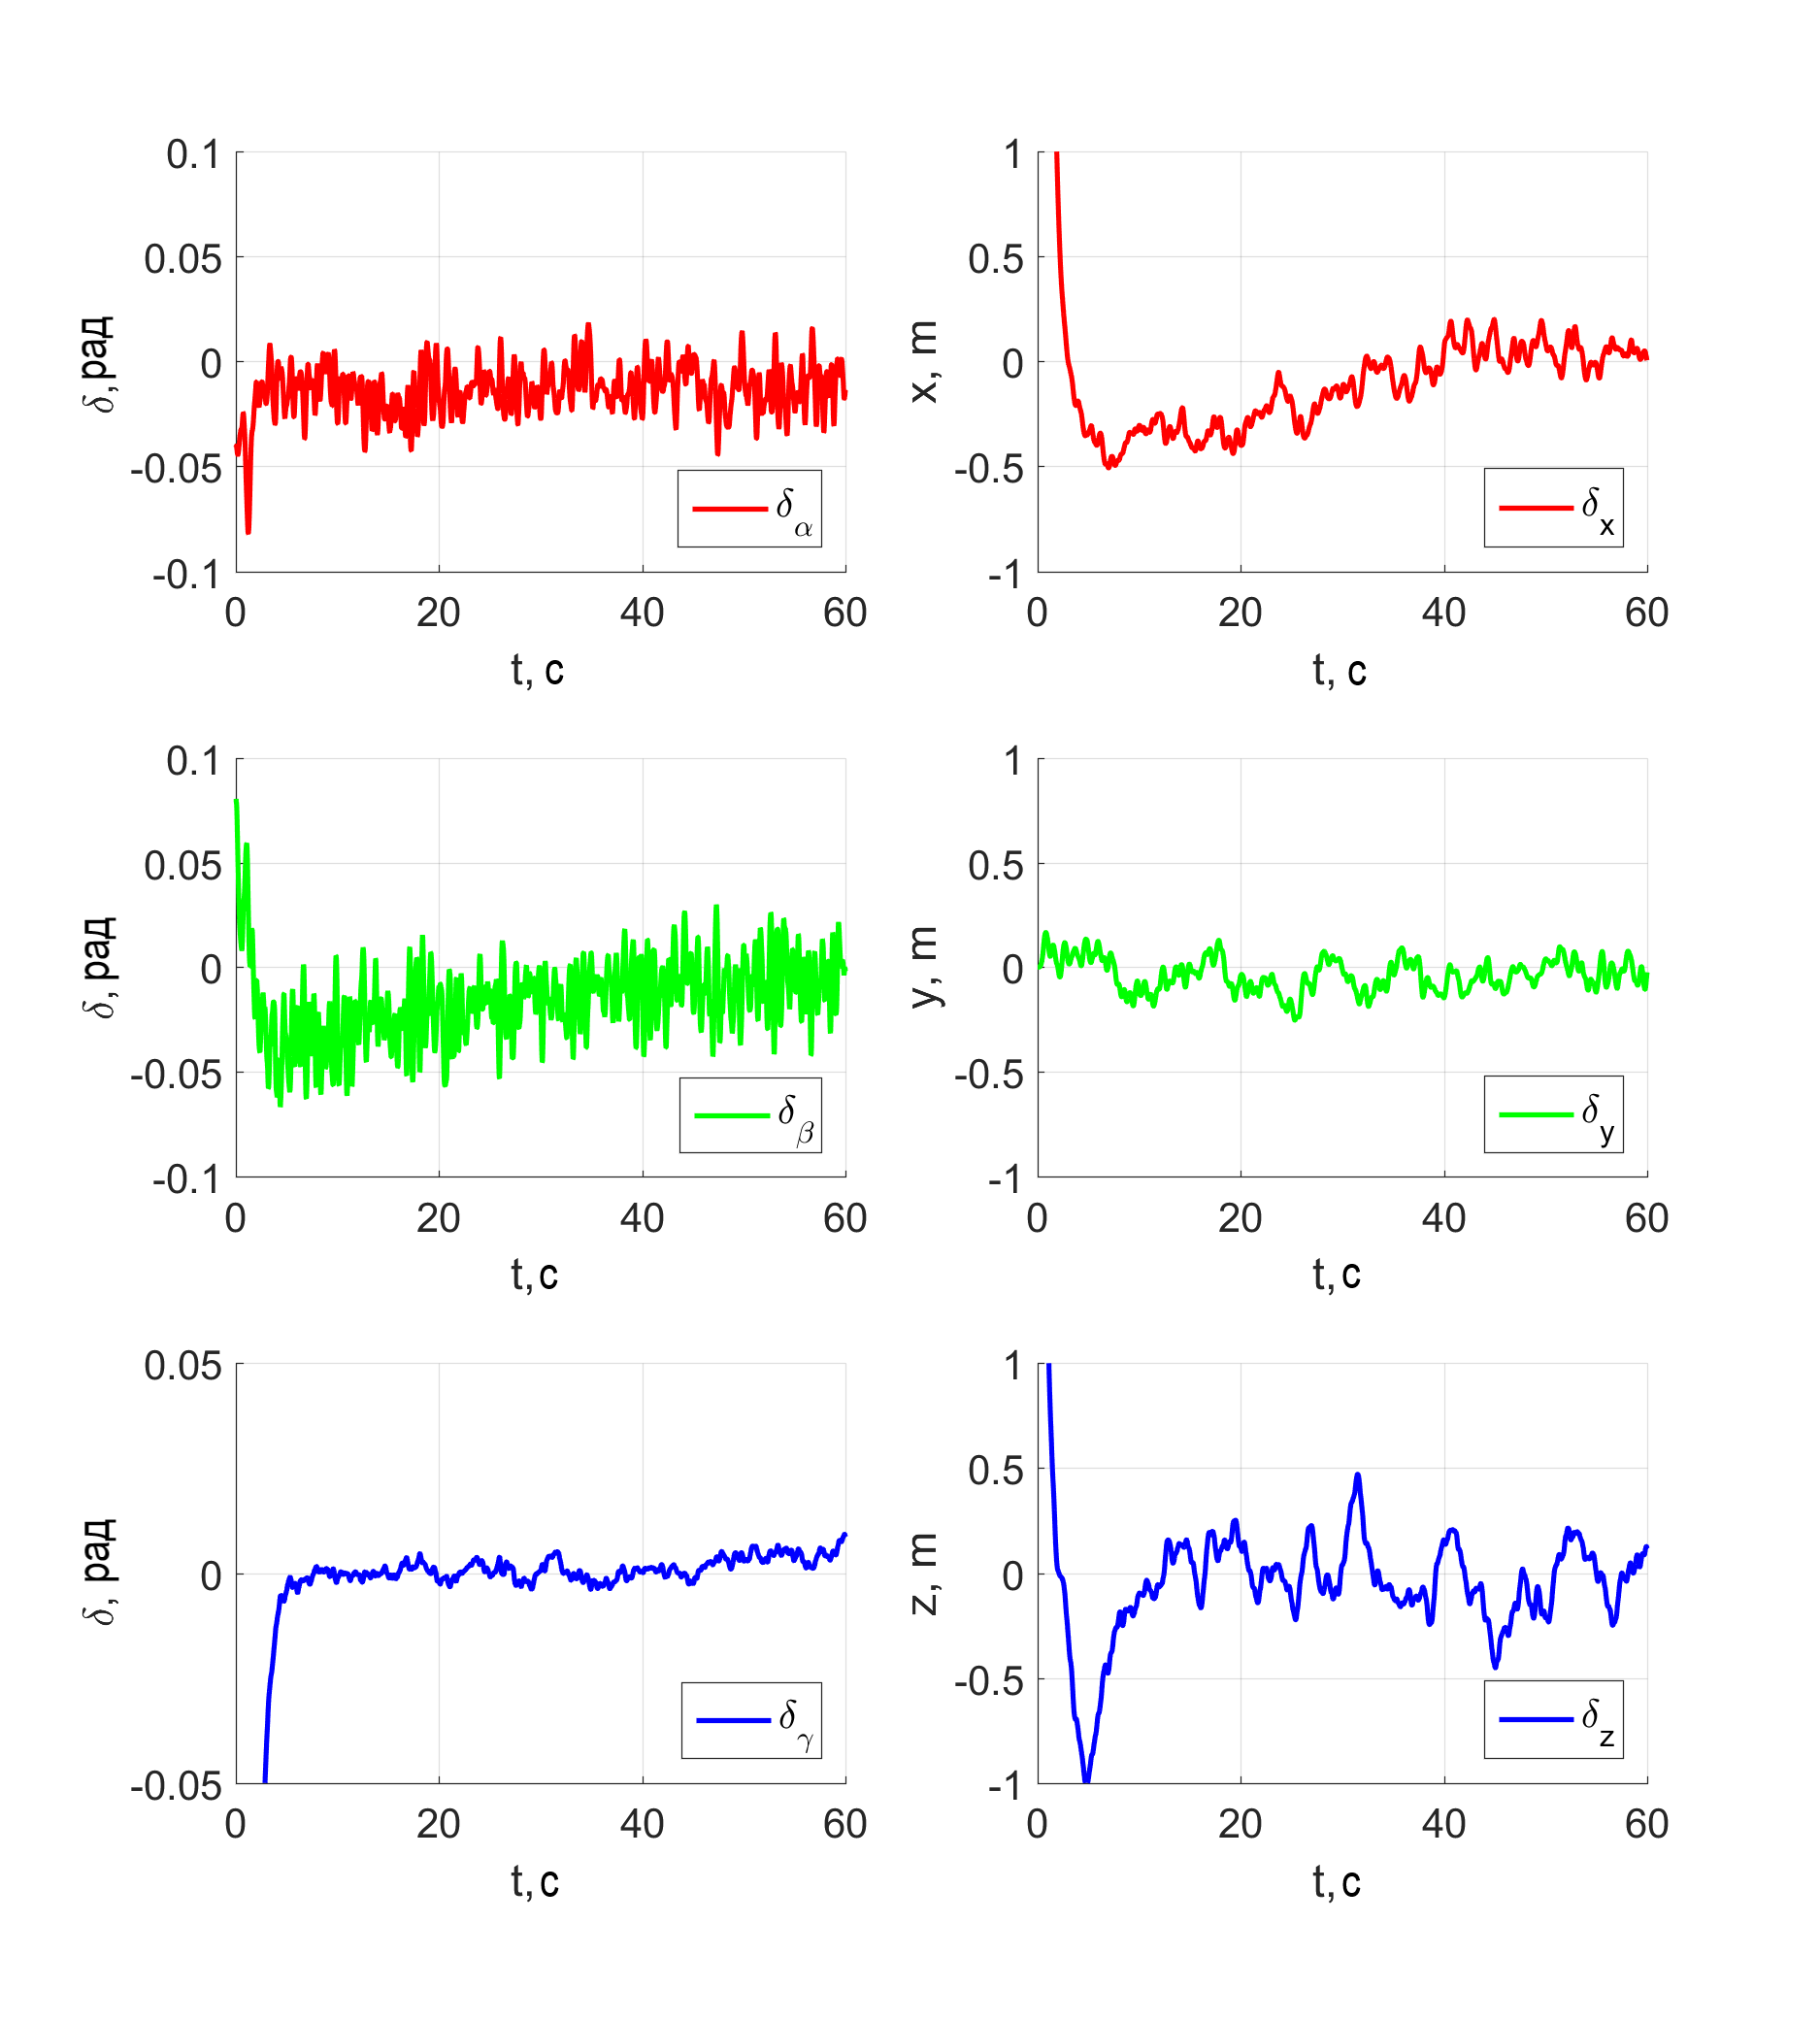
\includegraphics[width=14cm]{errors_rows.png}
	\caption{ -- Отклонение параметров движения БЛА от целевых значений}
	\label{fig:mau_errors}
\end{figure}

На рисунке \ref{fig:mau_cam} можно проследить за траекторией наблюдаемого объекта на записи, которою можно сделать с помощью передней камеры.
Видно, что в начальный момент времени объект находится вне зоны видимости, затем перемещается в центр экрана и далее на протяжении всего времени манёвра ось визирования камеры отклоняется от направления на объект не более чем на 1$^\circ$.
\begin{figure}[H]
	\centering
	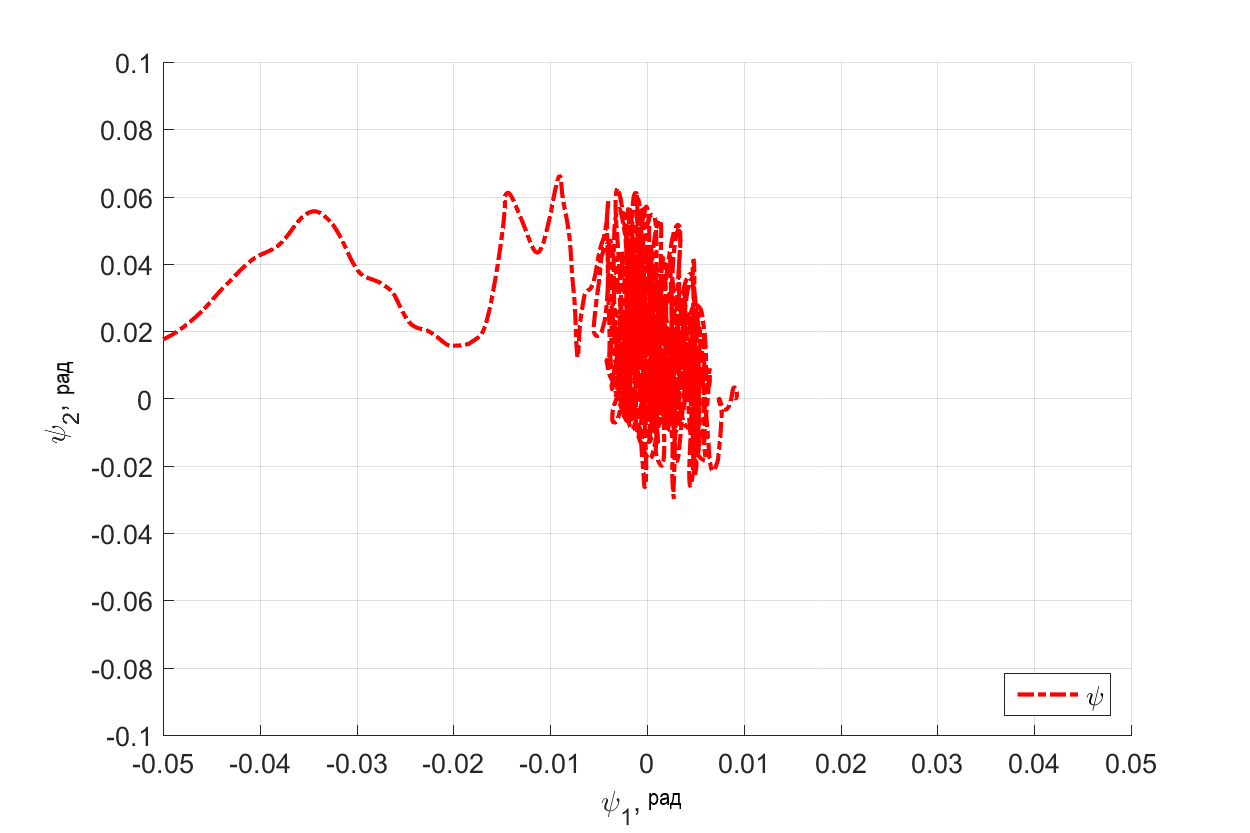
\includegraphics[width=14cm]{camera.png}
	\caption{ -- Траектория объекта на записи}
	\label{fig:mau_cam}
\end{figure}
Рисунок \ref{fig:mau_est} демонстрирует производительность кубатурного фильтра Калмана. Слева приведен график ошибки оценки угла крена и его прямых измерений, справа – оценка положения по оси $X$ и его прямые измерения.
Алгоритмы фильтрации позволили значительно понизить уровень шума измерений.
\begin{figure}[H]
	\centering
	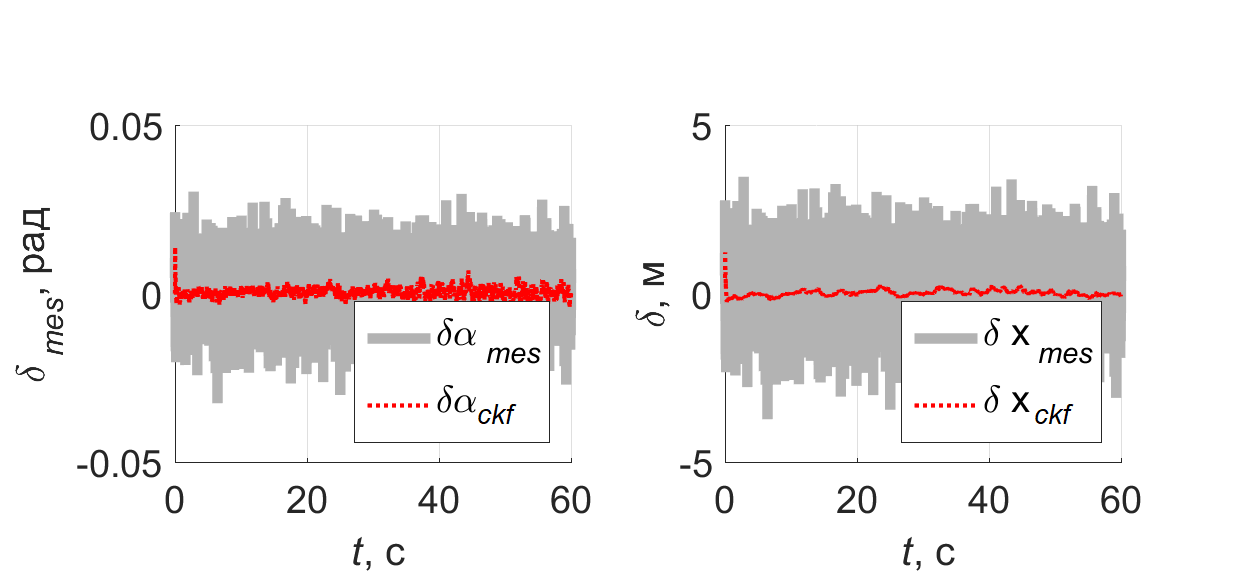
\includegraphics[width=14cm]{ckf_perf_raws_cut.png}
	\caption{ -- Ошибка оценки состояния и прямых измерений}
	\label{fig:mau_est}
\end{figure}

На графиках, изображенных на рисунке \ref{fig:mau_ctrl_out} представлены компоненты вектора управляющих параметров, которые лежат внутри ограниченной предельными значениями области.

\begin{figure}[H]
	\centering
	\subfloat{%
		\subfloat[]{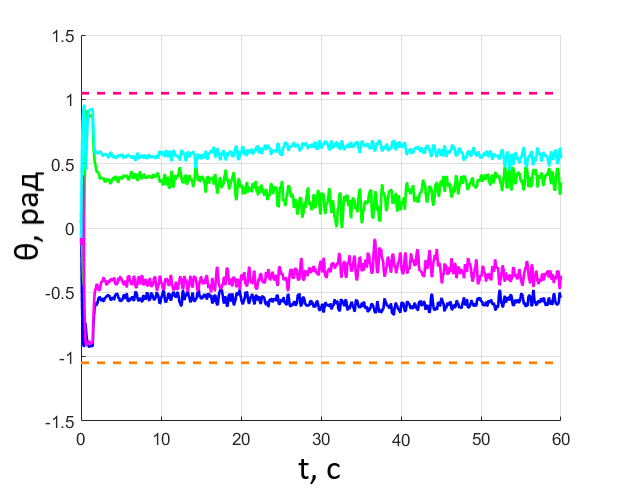
\includegraphics[clip,width=0.49\columnwidth]{rotor_angles}}%
		\subfloat[]{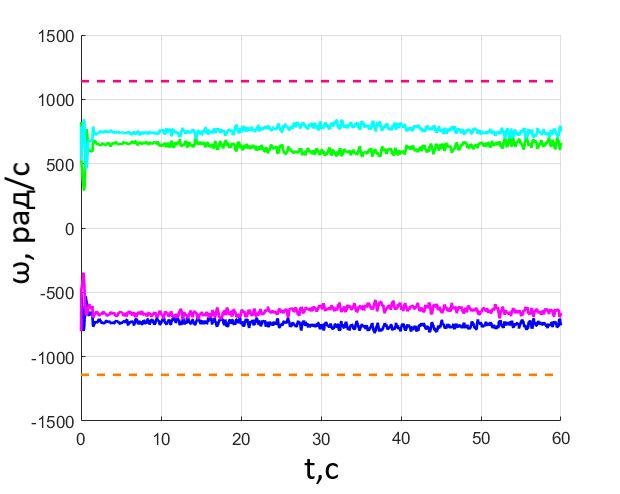
\includegraphics[clip,width=0.49\columnwidth]{rotor_rates}}%
	}
	
	\caption{ -- Управляющие параметры}
	\label{fig:mau_ctrl_out}
	
\end{figure}


В результате эксперимента мы оценили способность БЛА с поворотными роторами справляться со сложными маневрами, где необходимо независимо управлять ориентацией и положением аппарата. Квадрокоптер быстро вышел на целевую траекторию и успешно отслеживал ее, ориентируя бортовую камеру таким образом, чтобы объект наблюдения всегда оставался в центре изображения.

Во втором эксперименте рассматривается сценарий отказа двух смежных двигателей. Для возможности применения системы экстренного управления необходим значительный запас тяги двигателей и широкие пределы отклонений сервоприводов
\begin{equation}
\begin{aligned}
&\tilde{\omega}_{max} = 1318 рад/c,
\\
&\theta_{max} = \pi.
\end{aligned}
\end{equation}

В начальный момент времени аппарат находится на высоте 25 метров недалеко от точки взлета.
При отказе двигателей начинается переход в режим экстренного управления.
За время менее 5 секунд высота БЛА упала более чем на 15 метров, но затем, когда аппарат стабилизировал свою ориентацию около целевых значений, падение прекратилось и аппарат приступил к плавному снижению со скоростью около 0,5 метров в секунду с одновременным движением в сторону места своего запуска. По истечении 30 секунд квадрокоптер стабилизировал свое положение около точки взлета. На рисунке \ref{fig:em_coords} представлены параметры движения мультироторного робота в процессе экстренной посадки. Слева изображены графики компонент векторной части кватерниона ориентации корпуса, справа -- проекции координат центра масс БЛА на оси инерциальной системы отсчета.
\begin{figure}[H]
	
	\centering
	\subfloat[крен]{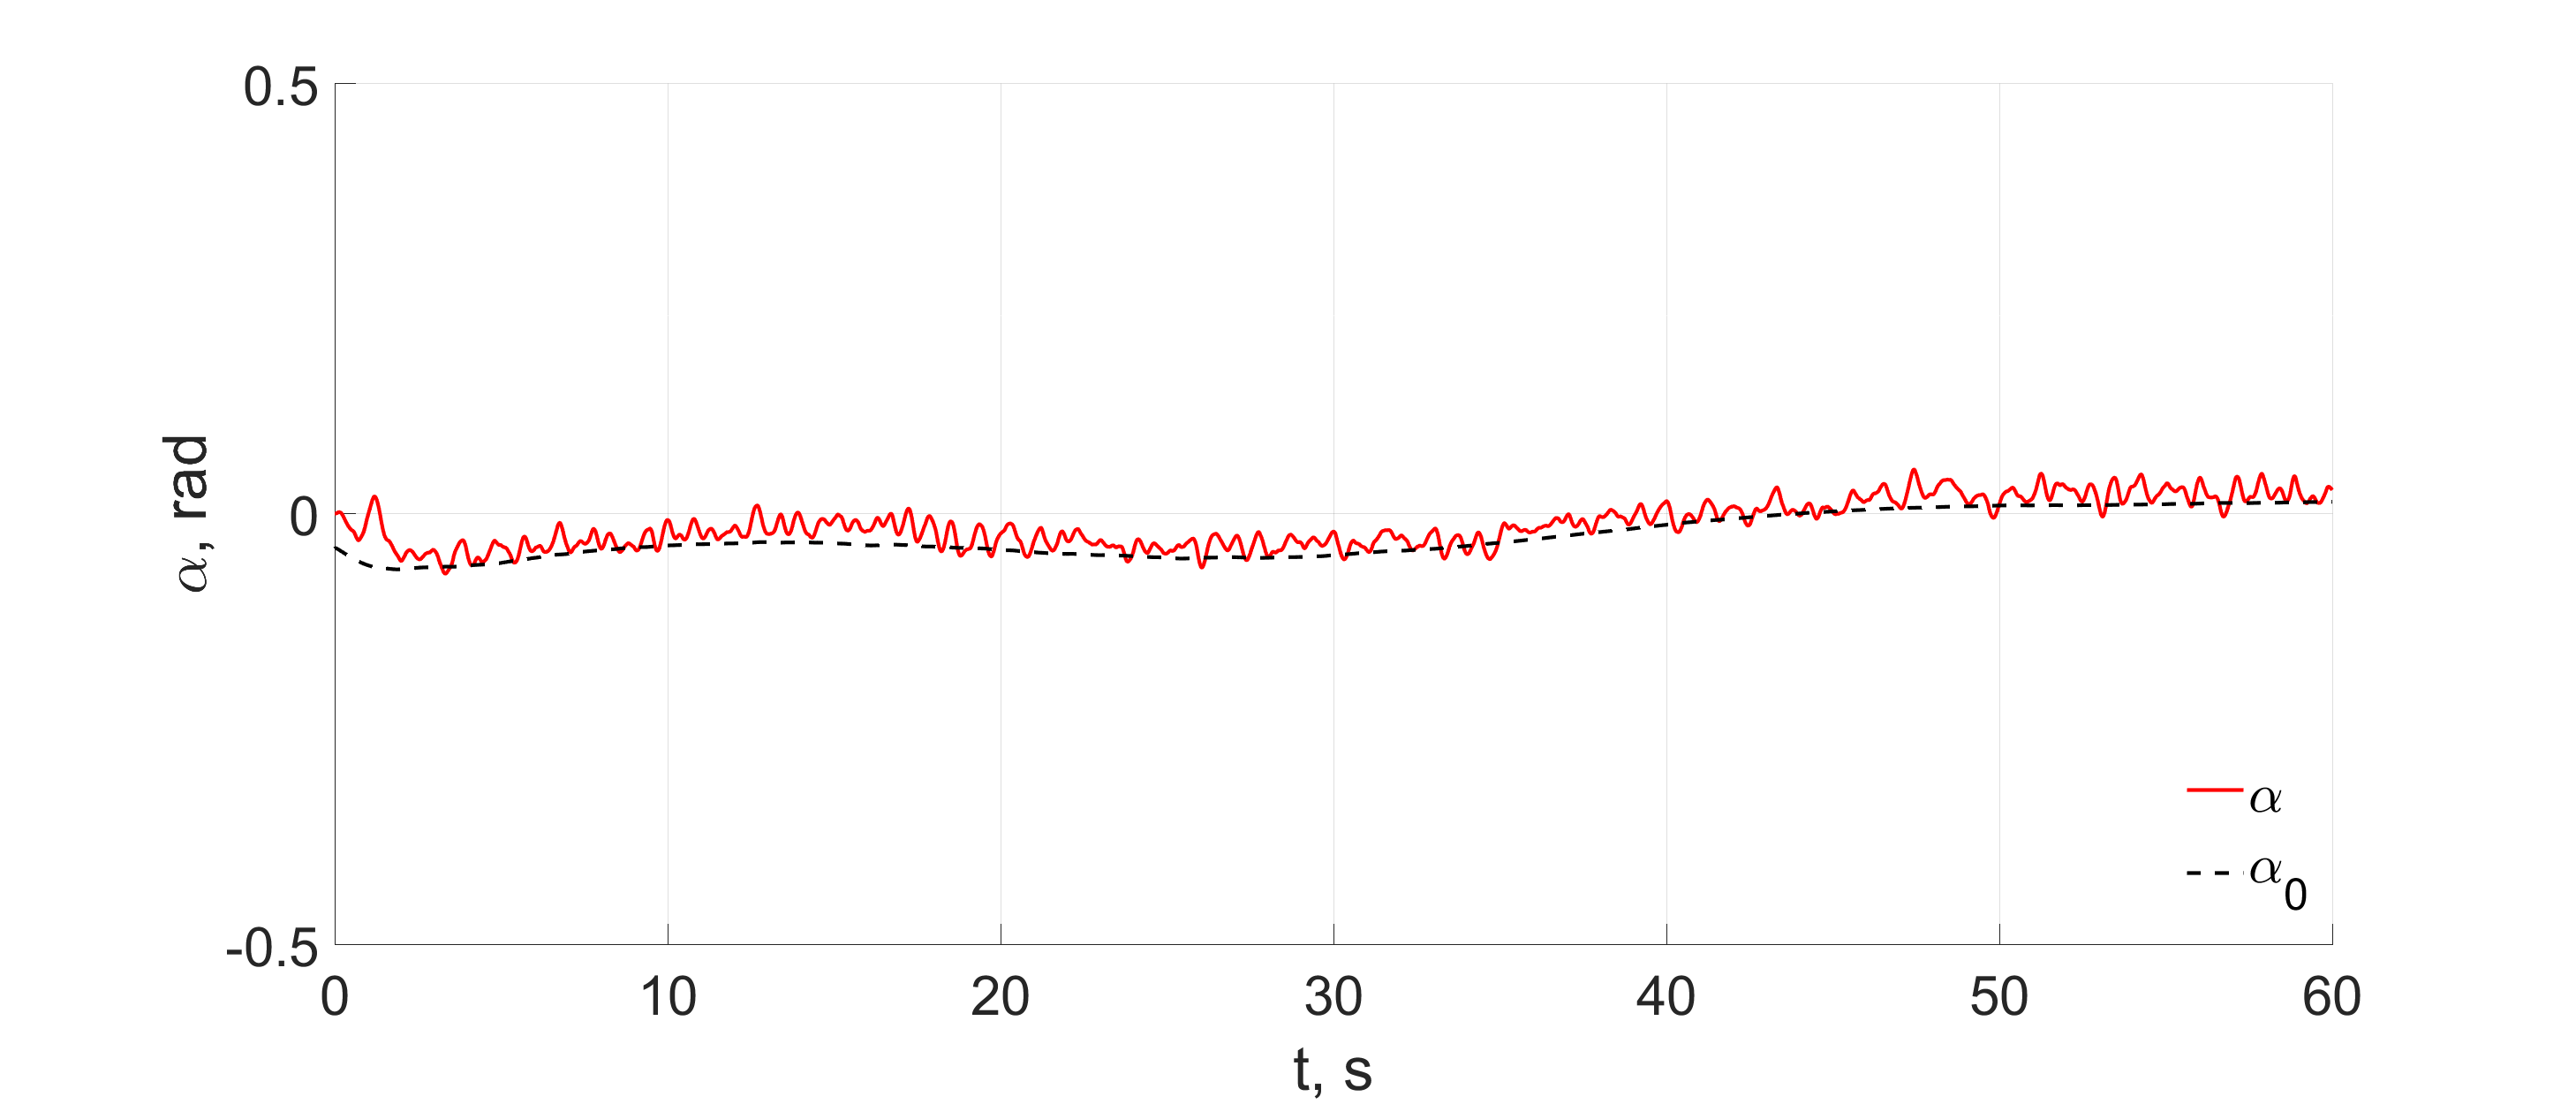
\includegraphics[width=7cm]{em/roll}}\hfil
	\subfloat[координата x]{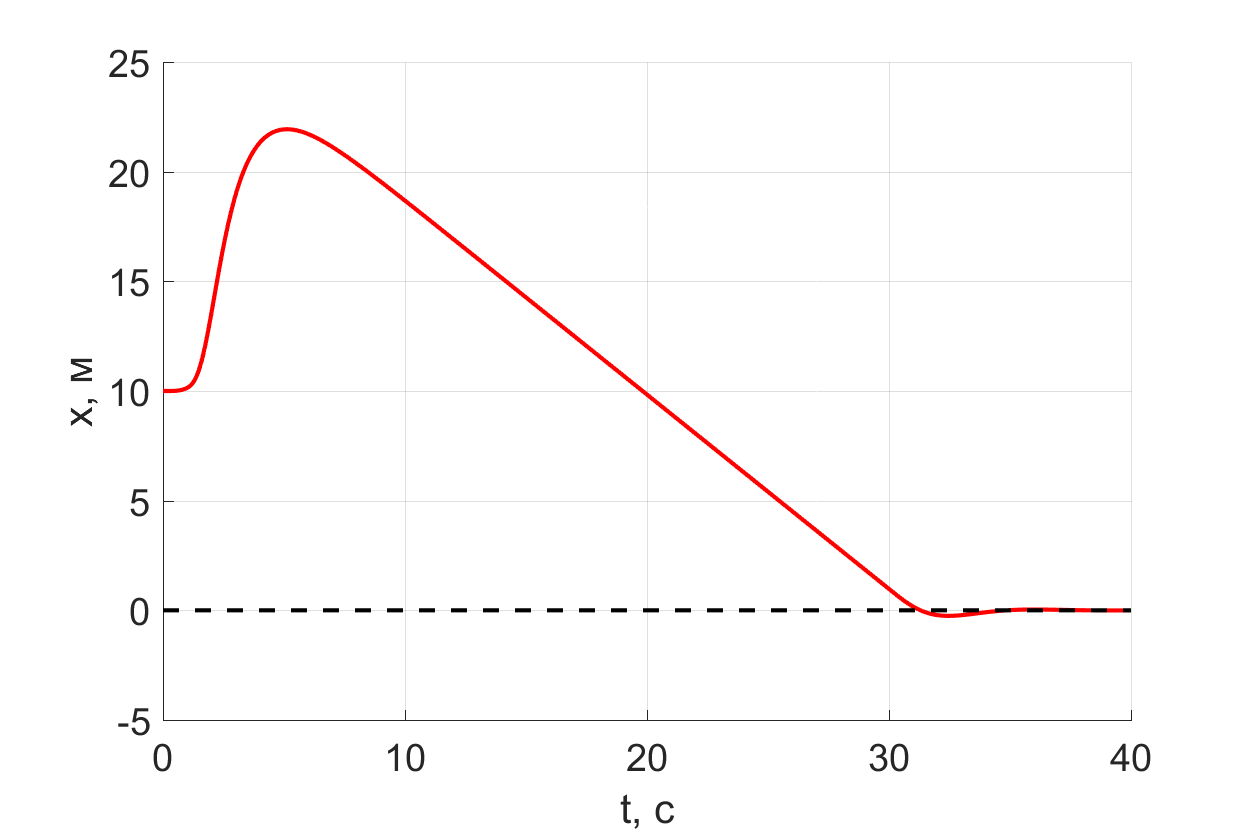
\includegraphics[width=7cm]{em/x}}
	
	\subfloat[тангаж]{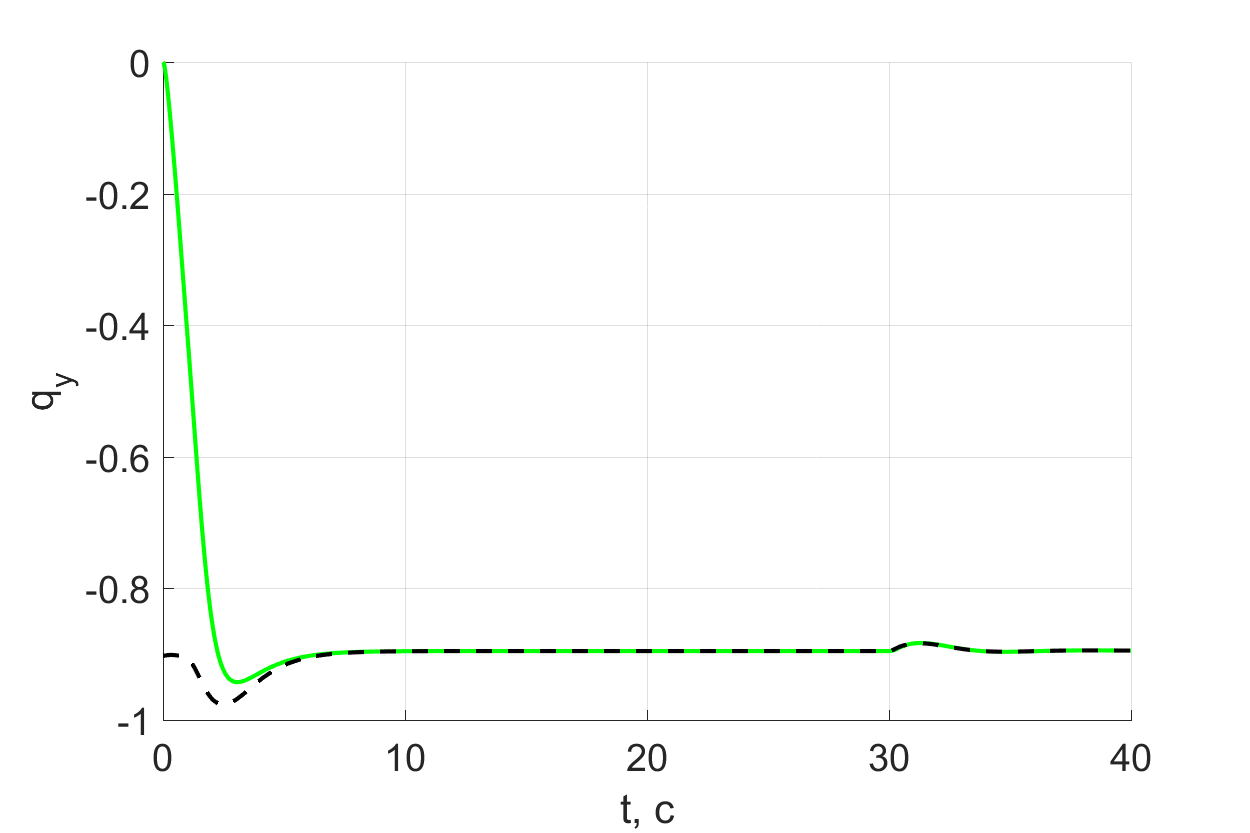
\includegraphics[width=7cm]{em/pitch}} \hfil 
	\subfloat[координата y]{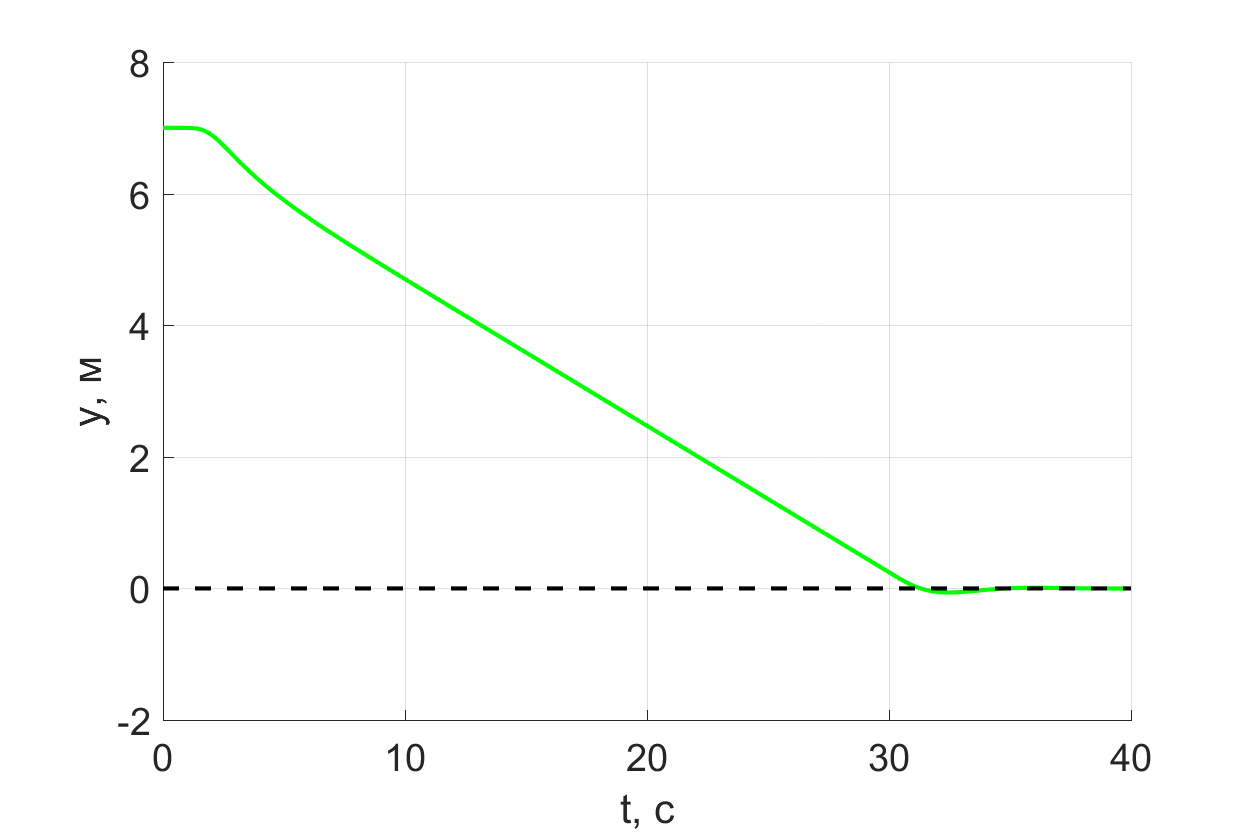
\includegraphics[width=7cm]{em/y}}  
	
	\subfloat[рысканье]{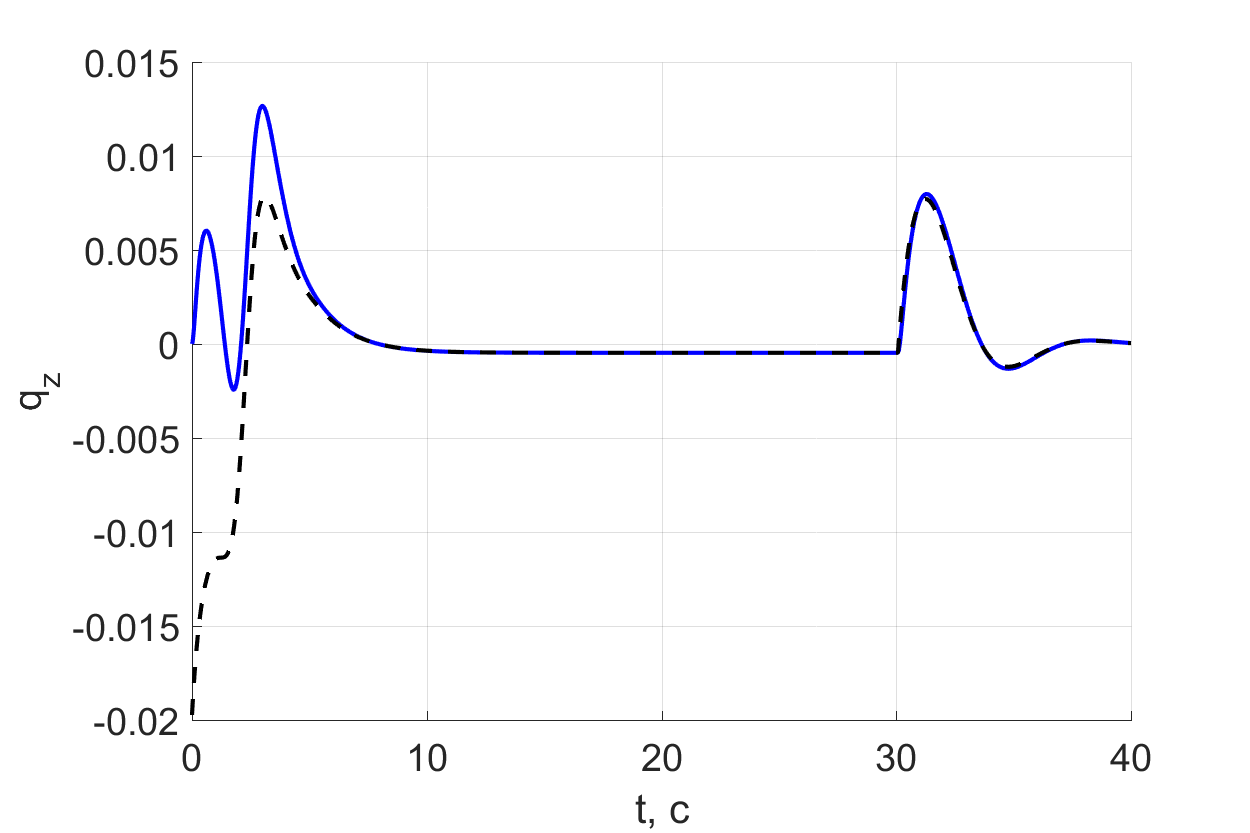
\includegraphics[width=7cm]{em/yaw}}\hfil
	\subfloat[координата z]{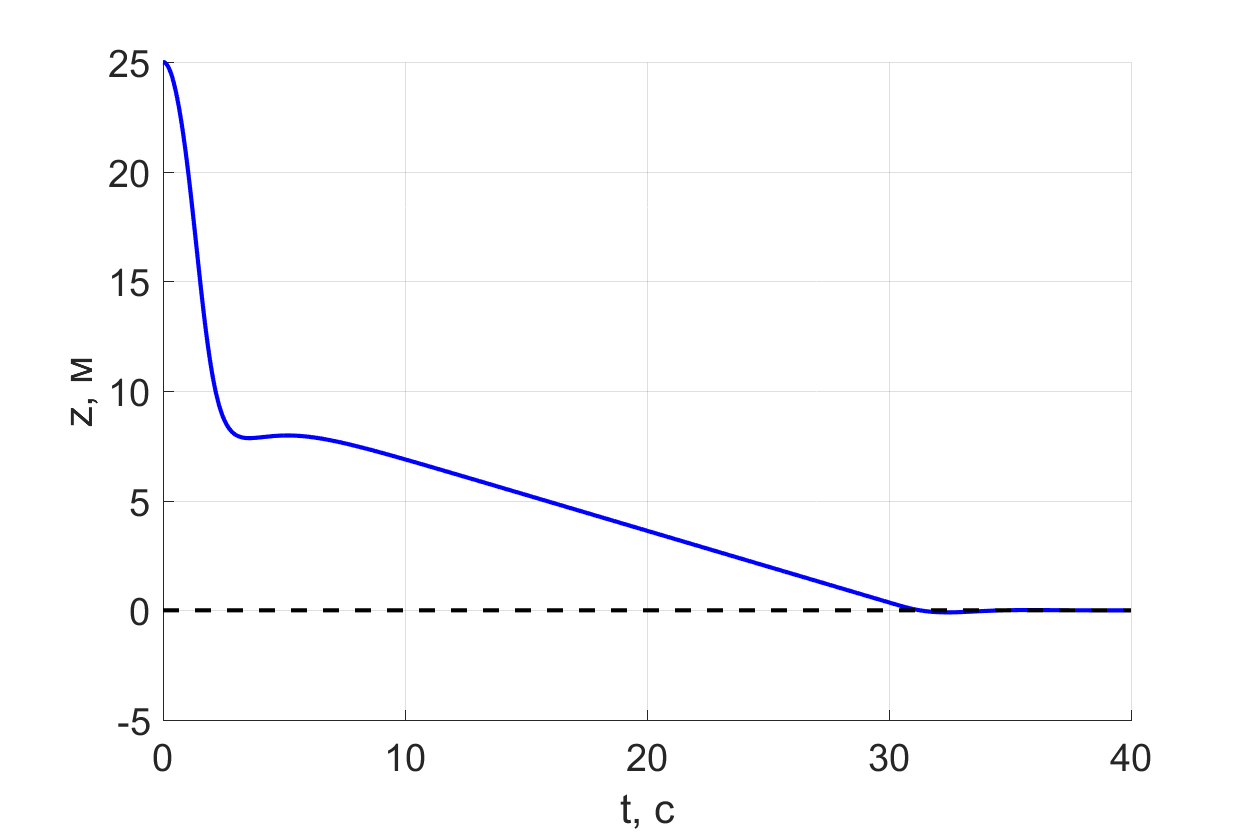
\includegraphics[width=7cm]{em/z}}
	\caption{ -- Параметры движения БЛА при экстренной посадке}
	\label{fig:em_coords}
\end{figure}

Таким образом было показано, что БЛА с поворотными роторами при соблюдении некоторых требований к параметрам исполнительных органов системы управления способен продолжить свое движение после отказа двух смежных двигателей.

\textbf{В заключении} приводятся основные результаты диссертационной работы:
\begin{enumerate}
	\item Разработана математическая модель управляемой динамики квадрокоптера с поворотными роторами с учётом сил и моментов, действующих на все составные части системы;
	\item  Получено аналитическое решение задачи обратной динамики БЛА с поворотными роторами;
	\item Синтезирован контур управления квадрокоптером с поворотными роторами для независимого управления положением и ориентацией; 
	\item Разработан алгоритм для учёта физических ограничений, накладываемых на исполнительные органы системы управления;
	\item Разработан алгоритм для идентификации основных параметров модели;
	\item Разработаны алгоритмы экстренного управления квадрокоптером с поворотными роторами в случае отказа двух смежных двигателей.
	\item Разработан полный набор алгоритмов системы управления квадрокоптером с поворотными роторами.
\end{enumerate}
